\documentclass{article}
\usepackage[T1]{fontenc}
\usepackage[landscape, margin=1in, papersize={9in, 12in}]{geometry}
\usepackage{fontspec, nopageno, xltxtra, xunicode}
\usepackage{lilyglyphs}
\usepackage{tikz}
\usepackage{hyperref}
\hypersetup{
    colorlinks=true,
    linkcolor=black,
    filecolor=magenta,
    urlcolor=black,
}% \usepackage{twocolumn}
% \usepackage{multicols}
\usepackage{vwcol}
\usepackage{lipsum}
\usetikzlibrary{arrows}
\usetikzlibrary{shapes}
\parindent=0pt
\parskip=12pt
\setmainfont{Adobe Garamond Pro}
\usepackage{booktabs}
\usepackage[normalem]{ulem}

\useunder{\uline}{\ul}{}
\begin{document}

\begin{center}
  {\Huge Performance Notes }
\end{center}

{\large Instrumentation}

\textit{Aristeia} is written for a solo percussionist playing three sets of three instruments.
Specific instrumentation is left up to the performer, within the following bounds:

\begin{itemize}
  \item All percussion is unpitched
  \item Each set of three instruments must be chosen from the same family, arranged in rough low to high order
  \item Each set of three must be from a different instrument family
  \item All instruments should be playable with the same beaters or mallets
  \item The sustain and decay for all instruments should be fairly quick
\end{itemize}

{\bf For example}, one possible instrumentation would be three toms, three wood blocks, and three table cymbals

\begin{center}
  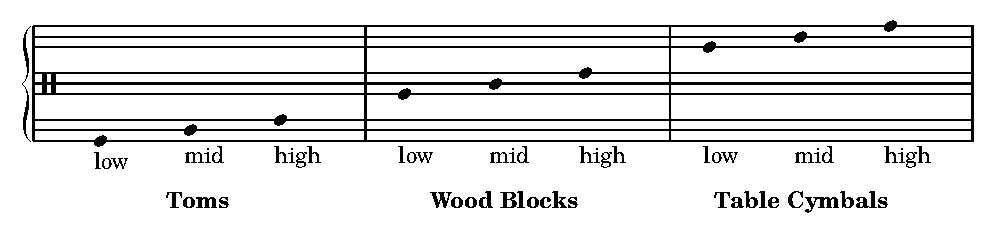
\includegraphics[scale=.8]{./instruments-cropped.pdf}
\end{center}

{\large Grace Notes}

Grace notes are always played before the beat, including grace notes that precede a rest.

\vspace{1.5em}
{\large Dynamics}

Dynamics in \textit{Aristeia} are notated in a range from \lilyDynamics{pp} to \lilyDynamics{ff}. These should be taken to define the desired sharpness of attack, rather than the resultant sound.
\pagebreak


{\large Articulations}

{\bf Marcato} signifies a noticeable accent.

{\bf Tenuto} signifies a slight accentuation of the note. This is meant to be felt by the player more than it is necessary for the audience to hear it.

No other notes should be accented. Meter in {\it Aristeia} is a function of phrasing and organization, not pulse.

\vspace{1.5em}
{\large Tuplets}

Tuplets are notated by a bracket and a single number, as below.

\begin{center}
  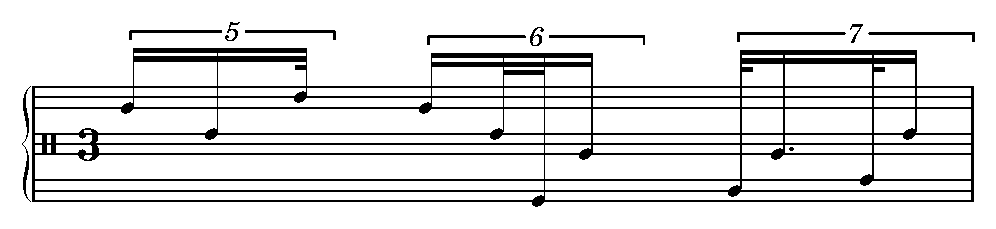
\includegraphics[scale=.8]{./tuplets-cropped.pdf}
\end{center}

Throughout \textit{Aristeia}, the tuplet number defines the number of 32nd notes to be played in the space of an eighth note.

That is, 
\includegraphics[scale=.8]{./tuplet1.pdf} should always be read as 
\includegraphics[scale=.8]{./tuplet2.pdf}

\vfill

\begin{center}

  \textit{* \hspace{1em} * \hspace{1em} *}
  \vspace*{1\baselineskip}
\end{center}

  In the conventions of epic poetry, the \emph{aristeia} (from the Greek word for ``excellence'') is a battle scene which describes a hero’s arc in which, often inspired by one of the gods, the hero prepares for battle, single-handedly takes on and defeats a significant number of opponents, and then returns — sometimes alive, sometimes dead — to his camp.

This piece describes four different but overlapping arcs. Each of the three collections of instruments has its own buildup and soloistic moment before retreating into the background, or disappearing. The interplay between these three arcs results in the performer’s own \emph{aristeia}, as the piece builds in intensity from its simple beginnings to its climax, and finally, a return — leaving the performer happily unharmed — to a reworking of the opening moments.

\end{document}
